\documentclass[a4paper,12pt]{article}
\usepackage[utf8]{inputenc}
\usepackage{graphicx}
\usepackage{amsmath}
\usepackage{float}
\usepackage{parskip}

\title{How has COVID impacted economic activity and what have been the extent of these impacts?}
\author{Terry Qi}

\begin{document}

\maketitle
\newpage
Word count:

Article: https://www.bbc.com/news/business-54186359, Covid pushes New Zealand into worst recession in years, 17/09/2020, published by the BBC, on 17/09/2020, accessed 27/10/2021

Topic Macroeconomics

Key Concept: Change


% planning
% gdp shrank 12.2% lockdown. first recession. impact on retail, accommodation, restaurations, transport, decline production travel bans.

% more research: inflation, unemployment, imports & exports, economic growth



% unemployment, suddenly peeked at 5.3% in third quarter of 2020, slowly growing in the first two quarters of the pandemic

% inflation, slowly increasing from the third quarter of  2019, decreases at the 2nd quarter in 2020.

% imports & exports, 

% economic growth: GDP.



% https://www.stats.govt.nz/information-releases/balance-of-payments-and-international-investment-position-june-2021-quarter

% https://www.stats.govt.nz/information-releases/consumers-price-index-september-2021-quarter

% https://www.stats.govt.nz/information-releases/labour-market-statistics-june-2021-quarter



\section*{Topic}
The article chosen discussed the impact of COVID-19 on the economy of New Zealand in 2020. It stated a measured 12.2\% decrease in the national nominal GDP, as well as classifying the status as ``the deepest recession in decades''. This discussion will focus on the change in the retail sectors of the economy through the application of economic theory, and will evaluate its broader impacts on the wider economy.

\section*{Theory}
Aggregate demand (AD), is defined as the summation of all the market demands in the economy, consisting of Consumption, Investment, Government Spending, and Net Exports. As stated in the article, the pandemic had directly affected the retail industry in a perceived decrease in production quantity. This is very likely caused by various international travel bans and strict nationwide lockdowns, restricting the demand from consumers and households, directly decreasing and changing the Consumption component of AD.

For analysis, the Keynsian model of the economy is used, for NZ have strong labor unions and regulations (citations), creating sticky wages as price levels decreases, fulfilling the assumptions of the Keynsian model. Additionally, the initial level of real output ($Y_1$) is drawn close to the level of full employment ($Y_f$), for average unemployment rates in the NZ is relatively low at around 4\% throughout 2020, thus lessening the recessionary gap, defined as $Y_f-Y_1$.

This is shown in figure \ref{fig:asad} through a leftwards shift of the aggregate demand from $AD_1$ to $AD_2$. The decreased aggregate demand will reduce the NZ real GDP (real output), for total expenditure and money flow will slow down from a lack of demand to do so, reducing real GDP from $Y_1$ to $Y_2$. Moreover, the small recessionary gap means that a moderate decrease in the price level is to be expected, from $PL_1$ to $PL_2$, because the decrease in real output creates vacancies in the demand of factors of productions, causing their owners to lower their cost/interest rates to maximize profit, thus lowering the cost of production and thus the price level.

Furthermore, 
 
 
% theory
\begin{figure}[H]
    \centering
    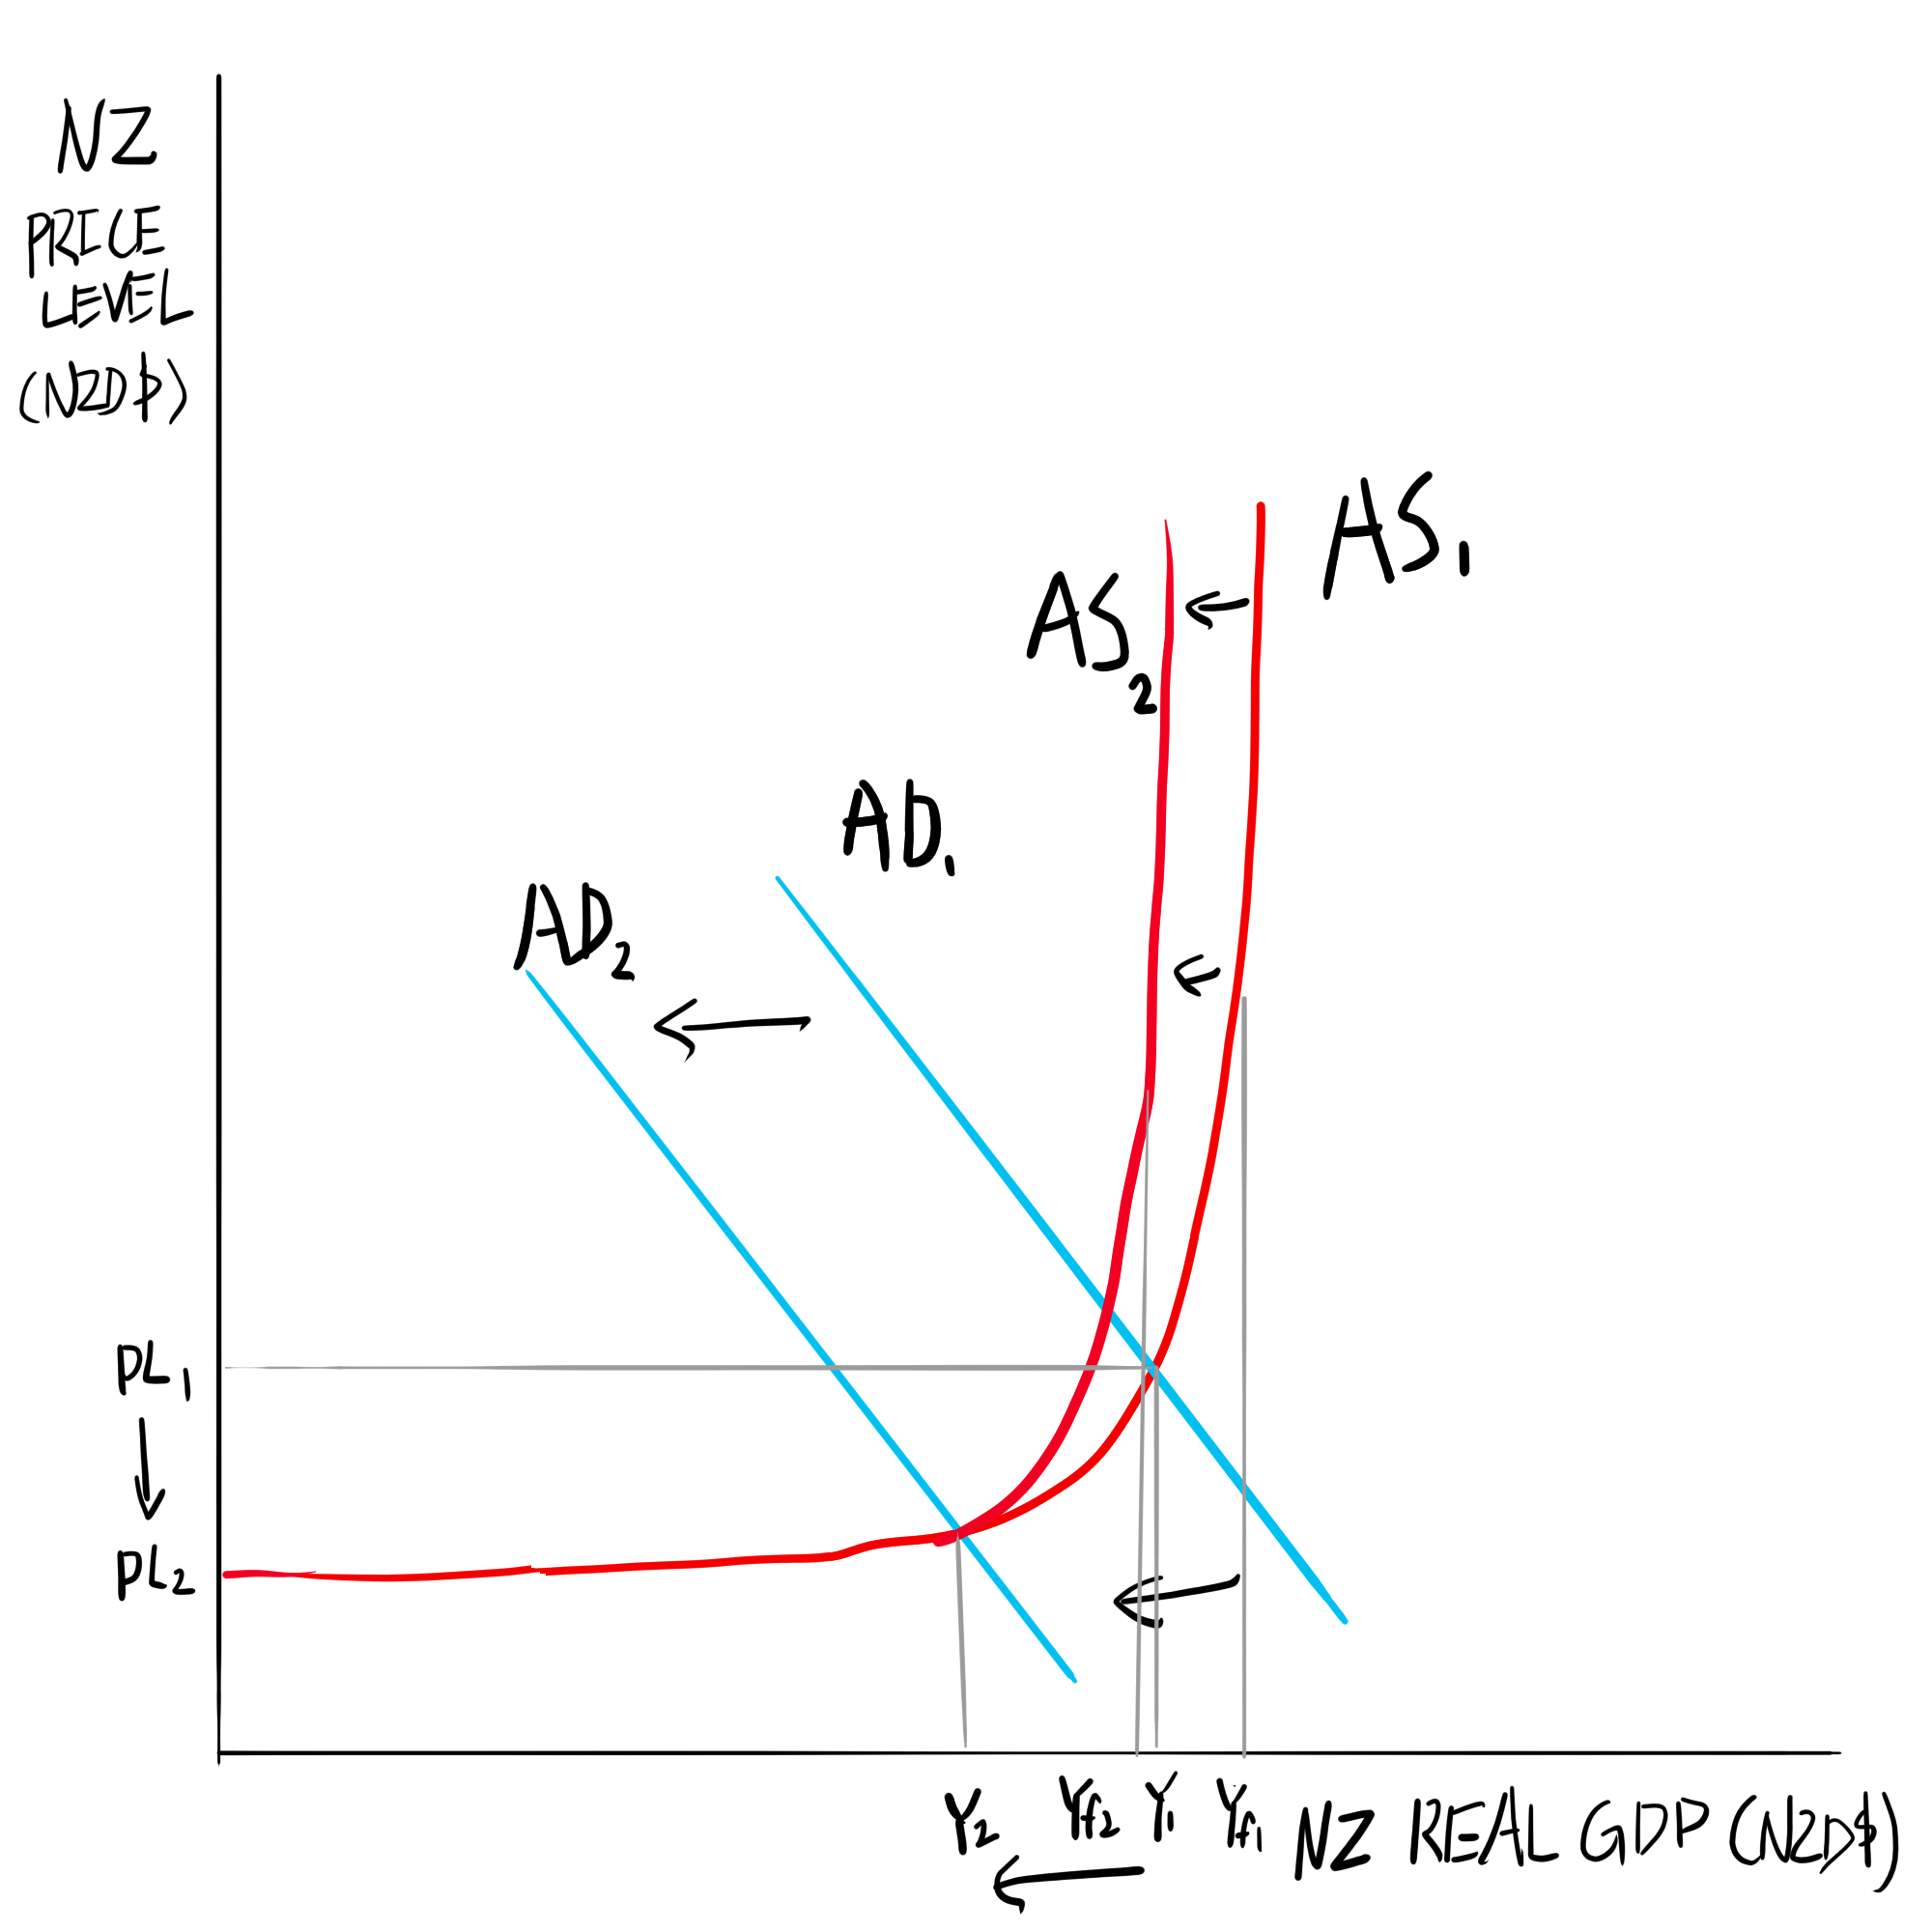
\includegraphics[scale=0.6]{assets/asad.png}
    \caption{The NZ economic diagram during COVID}
    \label{fig:asad}
\end{figure}

\section*{Evaluation}

% more stuff

\section*{Summary}

% end

\end{document}
